\chapter{Relativit\`a Einsteniana}
\minitoc
% Einstein affermava che $c$ era una costante universale. Osservando
% che $x$ e $ct$ hanno le stesse unit\`a di misura, si potrebbe
% asserire che non sono pi\`u $\Delta x$ e $\Delta t$ ad essere
% invarianti, bens\`i:
% \begin{equation}
%(\Delta s)^2 = (c\,\Delta t)^2-\Delta x^2. \label{eq:invariante}
%\end{equation}
%Che ci\`o sia invariante lo dimostreremo pi\`u avanti.
Einstein a questo punto si premura di costruire il suo sistema basato
su \ding{202}, \ding{203}, \ding{204}. Come comincia? Prendiamo una
sbarra lunga $l$ in un sistema di riferimento inerziale, che chiamiamo
$S$. Per prima cosa Einstein asserisce che assumere che ogni sistema
di riferimento inerziale veda la sbarra lunga $l$ non \`e, a priori,
un'ipotesi giustificata. Come si misura la lunghezza in moto? Per
concretizzare prendiamo una sbarra $\overline{PQ}$, solidale con il
sistema $S$, il quale si muove con velocit\`a $\mathbf{\mathsf{v}}$
rispetto al sistema $S'$; l'osservatore della sbarra misura la
lunghezza della sbarra con un metro (la sbarra \`e ferma rispetto a
lui); l'osservatore in $S'$ pu\`o fotografare la sbarra e misurare la
fotografia, di modo che gli estremi $P$ e $Q$ siano osservati allo
stesso istante nel suo sistema di riferimento. Si ha che 
\begin{displaymath}
\begin{array}{l} S' \mbox{ dice che la sbarra misura } l'\\
  S \mbox{ dice che la sbarra misura } l \end{array}
\end{displaymath}

Einstein afferma che nulla, dal punto di vista logico, mi garantisce
$l=l'$. Quindi non \`e affatto detto che le misure di lunghezza
rimangano inviariate passando da un sistema di riferimento all'altro.
\section{Glory \& Consequences}
Diamo innanzi tutto la definizione di evento:
\begin{definizione}
  Gli eventi, dal punto di vista fisico, sono le minime determinazioni
  spazio-temporali possibili; un evento, nei diagrammi
  spazio-temporali \`e rappresentato da una coordinata spaziale
  (saranno $(x^1,x^2,x^3)$), ed una coordinata temporale (sar\`a
  indicata come $x^0$).%
  \footnote{Dato che non sono capace di disegnare
    in 4-D, e d'altronde voi non siete capaci di vedere in 4-D
    (eccetto Candilera), sopprimiamo dai nostri disegni le altre due
    coordinate spaziali, con le quali siamo abituati a trattare.}
\end{definizione}
La metrica spazio-temporale per questi eventi sar\`a
\begin{equation}
  \label{eq:invariante}
  \de s^2 = \de t^2 - \de \bef{x}^2
\end{equation}
Prendiamo in considerazione un diagramma (vedi figura
\ref{fig:diagramma1}) dove come ascisse abbiamo le $x$, e come
ordinate abbiamo $ct$. I diagrammi che andremo a considerare
descriveranno dunque lo spazio tempo, assumendo che esso sia una
variet\`a differenziale a 2 (o a 4) dimensioni \footnote{Ovvero esso
  \`e continuo, differenziabile, con topologia localmente omeomorfa ad
  $\mathbb{R}^2$, o $\mathbb{R}^4$, separabile, con base di intorni
  numerabile (e pu\`o perci\`o essere metrizzabile).}. Tali diagrammi,
detti diagrammi di Minkowski\index{Minkowski!diagrammi di},
rappresentano lo spazio quadridimensionale con la metrica data dalla
(\ref{eq:invariante}), e questo spazio fornito di tale metrica \`e
detto spazio di Minkowski\index{Minkowski!spazio di}. In questo
diagramma tutti i raggi di luce che vi vengono rappresentati, sono
inclinati di $45^{\circ}$, poich\'e $c = x / t$. La traiettoria del
fascio di luce deve quindi essere la bisettrice tra asse spaziale ed
asse $ct$.\footnote{Come conseguenza del fatto che la velocit\`a della
  luce \`e uguale in tutti i sistemi.} Consideriamo un corpo~$A$ e un
corpo~$B$. L'origine sia $O$. $A$ e $B$ abbiano distanze uguali
rispetto ad $O$. Si faccia riferimento alla figura
\ref{fig:diagramma1}

\begin{figure}[htbp]
  \begin{center}
    \psfrag{ct}{$ct$} \psfrag{A}{$A$} \psfrag{B}{$B$} \psfrag{O}{$O$}
    \psfrag{x}{$x$}
    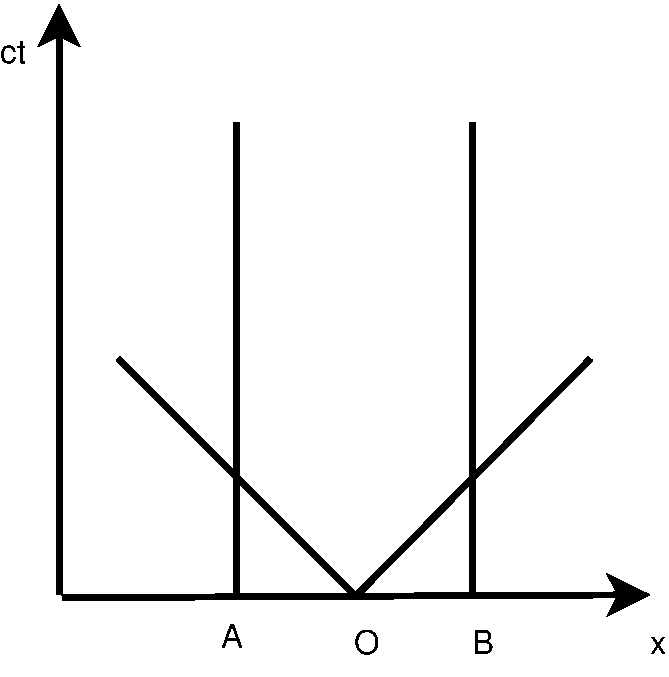
\includegraphics[height=7cm]{diagramma1.pdf}
    \caption{Traiettoria di due punti fermi colpiti da un raggio di
      luce} \label{fig:diagramma1}
  \end{center}
\end{figure}
Se i due corpi sono fermi le loro traiettorie sono rette parallele a
$ct$. Un raggio di luce che parte da $O$, li colpisce allo stesso
istante se $\overline{AO}=\overline{OB}$, come gi\`a assunto. Cambiamo
ora le cose. Siano i due corpi in moto con velocit\`a
$\mathbf{\mathsf{v}}$ rispetto ad $S$ (siano cio\`e solidali ad un
sistema $S'$). %Si ha che valgono le (\ref{eq:trasformazioni}).

\begin{figure}[htbp]
  \begin{center}
    \psfrag{ct}{$ct$} \psfrag{ct'}{$ct'$} \psfrag{A}{$A$}
    \psfrag{B}{$B$} \psfrag{O}{$O$} \psfrag{A'}{$A'$}
    \psfrag{B'}{$B'$} \psfrag{x'}{$x'$} \psfrag{x}{$x$}
    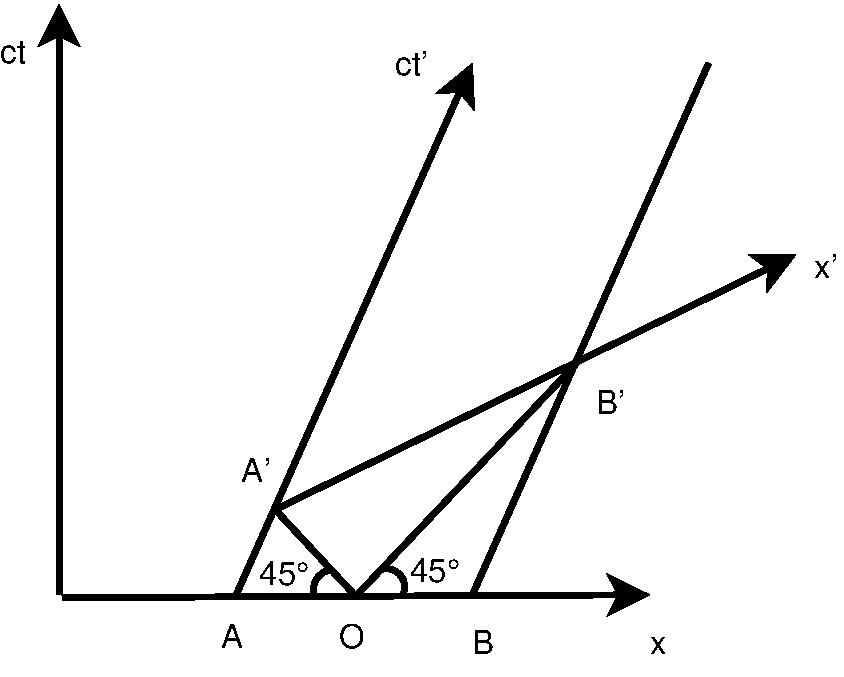
\includegraphics[height=7cm]{diagramma2.pdf}
    \caption{Traiettoria di due punti in movimento colpiti da un
      raggio di luce} \label{fig:diagramma2}
  \end{center}
\end{figure}
Facendo riferimento alla figura \vref{fig:diagramma2}, siano $A'$ e $
B' $ solidali a $ S' $, immagini di $A$ e $B$ t.c. $ \overline{ AO } =
\overline{ OB } $.  Per $ S' $ la situazione \`e uguale a quella vista
in precedenza, e dunque gli aventi $ A' $ e $ B' $ sono simultanei in
$ S' $; infatti la luce interseca la linea di universo di $ A' $ e di
$ B' $ (che sono le stesse di $ A $ e $ B $, ma ritorneremo su questo
nel paragrafo \vref{assoluto}) nello stesso $ t' $ (usando \ding{203}
e \ding{204}). In $ S' $, tuttavia i due eventi non sono pi\`u
simultanei (basta proiettarli sull'asse $ ct $ per
accorgersene). Allora:
\begin{osservazione}
  Eventi contemporanei in un sistema possono non esserlo in un altro
  sistema.
\end{osservazione}
\section{Le trasformazioni di Lorentz}
Riprendiamo il discorso del capitolo precedente da un punto di vista
algebrico. Come prima sia $S'$ sistema di riferimento inerziale in
moto con velocit\`a $\mathbf{\mathsf{v}}$ rispetto ad $S$. Tempi e
moti con gli apici si riferiscono ad $S'$; senz'apici ad $S$.

Consideriamo la traiettoria di un moto fermo in $S'$: $x'=x_{0}'$,
indipendentemente da $t'$. Tale moto in $S$ soddisfer\`a la relazione
$x-\mathsf{v}t=x_{0}$, con $x_{0}$ indipendente da~$t$.  Allora,
dacch\'e $x_{0}$ e $x_{0}'$ sono costanti rispetto a~$t$, si pu\`o
scrivere:
\begin{equation}
  \frac{x-\mathsf{v}t}{x'}=\alpha \quad\mbox{ costante.}
  \label{eq:lore1}
\end{equation}
Da qui ricavo $\alpha x'=x-\mathsf{v}t$. Per reciprocit\`a, scambiando
$S$ con $S'$ e $\mathsf{v}$ con $-\mathsf{v}$, ottengo:
\begin{equation}
  \frac{x'+\mathsf{v}t'}{x}=\alpha \label{eq:lore2}
\end{equation}
Combinando la (\ref{eq:lore1}) con la (\ref{eq:lore2}), in modo da
eliminare $x'$:
\begin{equation}
  t'=\frac{1}{\alpha}\left(t+\frac{\alpha^2-1}{\mathsf{v}}x\right)
  \label{eq:lore3}
\end{equation}
Se impongo che $t=t'$ ottengo $\alpha=1$ e $x'=x-\mathsf{v}t$.
Tuttavia per avere la relativit\`a ristretta non devo imporre
$\alpha=1$, bens\`i $c=\mathrm{costante}$, cio\`e $x'=ct'$ e
$x=ct$. Sostituendo quest'ultime relazioni dentro (\ref{eq:lore1}) e
dentro (\ref{eq:lore2}) ottengo:
\begin{displaymath}
  \alpha c t'=ct-\mathsf{v}t
\end{displaymath}
\begin{displaymath}
  \alpha ct=ct'+\mathsf{v}t'
\end{displaymath}
Facendo il prodotto tra le due ottengo
\begin{displaymath}
  \alpha=\pm \sqrt{1-\frac{\mathsf{v}^2}{c^2}}
\end{displaymath}
Dacch\'e per $v=0$ si ha $\alpha=1$, alla fin fine:
\begin{displaymath}
  \alpha=\sqrt{1-\frac{\mathsf{v}^2}{c^2}}
\end{displaymath}
Posso dunque ricavare le equazioni
\begin{displaymath}
  \left\{\begin{array}{l}
      x'=\frac{x-\mathsf{v}t}{\sqrt{1-\frac{\mathsf{v}^2}{c^2}}}\qquad
      \mbox{
        (deriva da (\ref{eq:lore1}))}\\
      \mbox{ }\\
      t'=\frac{t-\frac{\mathsf{v}x}{c^{2}}}{\sqrt{1-\frac{\mathsf{v}^2}{c^2}}}
      \qquad\mbox{ (deriva da (\ref{eq:lore3}))}
    \end{array}\right.
\end{displaymath}
Se introduciamo gli assi $x$ e $ct$ otteniamo le trasformazioni di
Lorentz \index{trasformazioni!di Lorentz}
\begin{equation}
  \left\{\begin{array}{l}
      x'=\frac{x-\frac{\mathsf{v}}{c}ct}{\sqrt{1-\frac{\mathsf{v}^2}{c^2}}}
      \\
      \mbox{ }\\
      ct'=\frac{ct-\frac{\mathsf{v}x}{c}}{\sqrt{1-\frac{\mathsf{v}^2}{c^2}}}
    \end{array}\right.\label{eq:Lorentz}
\end{equation}
A questo punto possiamo dimostrare che l'intervallo spazio temporale
$s^2$ \`e invariante
\begin{eqnarray*}
  (x')^2 - (ct')^2 & = &
  \frac{1}{1-\frac{\mathsf{v}^2}{c^2}}
  \left[(x-\mathsf{v}t)^2-(ct-\frac{\mathsf{v}}{c}x)^2\right]\\
  & = & x^2-(ct)^2
\end{eqnarray*}
Perci\`o se pongo $(c\;dt)^2-x^2=$cost, ne esce l'equazione di un
iperbole, e \emph{cost \`e la stessa per tutti i sistemi di
  riferimento inerziali.} Una volta trovate le (\ref{eq:Lorentz}) ci
accorgiamo che esse valgono per velocit\`a minori strettamente di
$c$. Infatti guardando il denominatore delle trasformazioni, ci
accorgiamo che deve valere la relazione:
\begin{displaymath}
  1-\frac{\mathsf{v}^2}{c^2}>0
\end{displaymath}
\begin{displaymath}
1-\frac{\mathsf{v}^2}{c^2}>0\qquad\Longrightarrow
c^2-\mathsf{v}^2>0\Longrightarrow c>v
\end{displaymath}
Quindi le trasformazioni \index{trasformazioni!di Lorentz}di Lorentz
connettono solo particelle che hanno velocit\`a strettamente minore di
$c$.

Riprendiamo per un attimo la discussione sulla quantit\`a inviarante
prima trovata. A seconda che la costante sia maggiore, minore, o
uguale a $0$ si hanno le situazioni in figura
\ref{fig:iperboli}.\newline
\begin{figure}[tb]
  \begin{center}
    \psfrag{ds^2=0}{$\Delta s^2 = 0$} \psfrag{ds^2>0}{$\Delta s^2 >
      0$} \psfrag{ds^2<0}{$\Delta s^2 < 0$}
    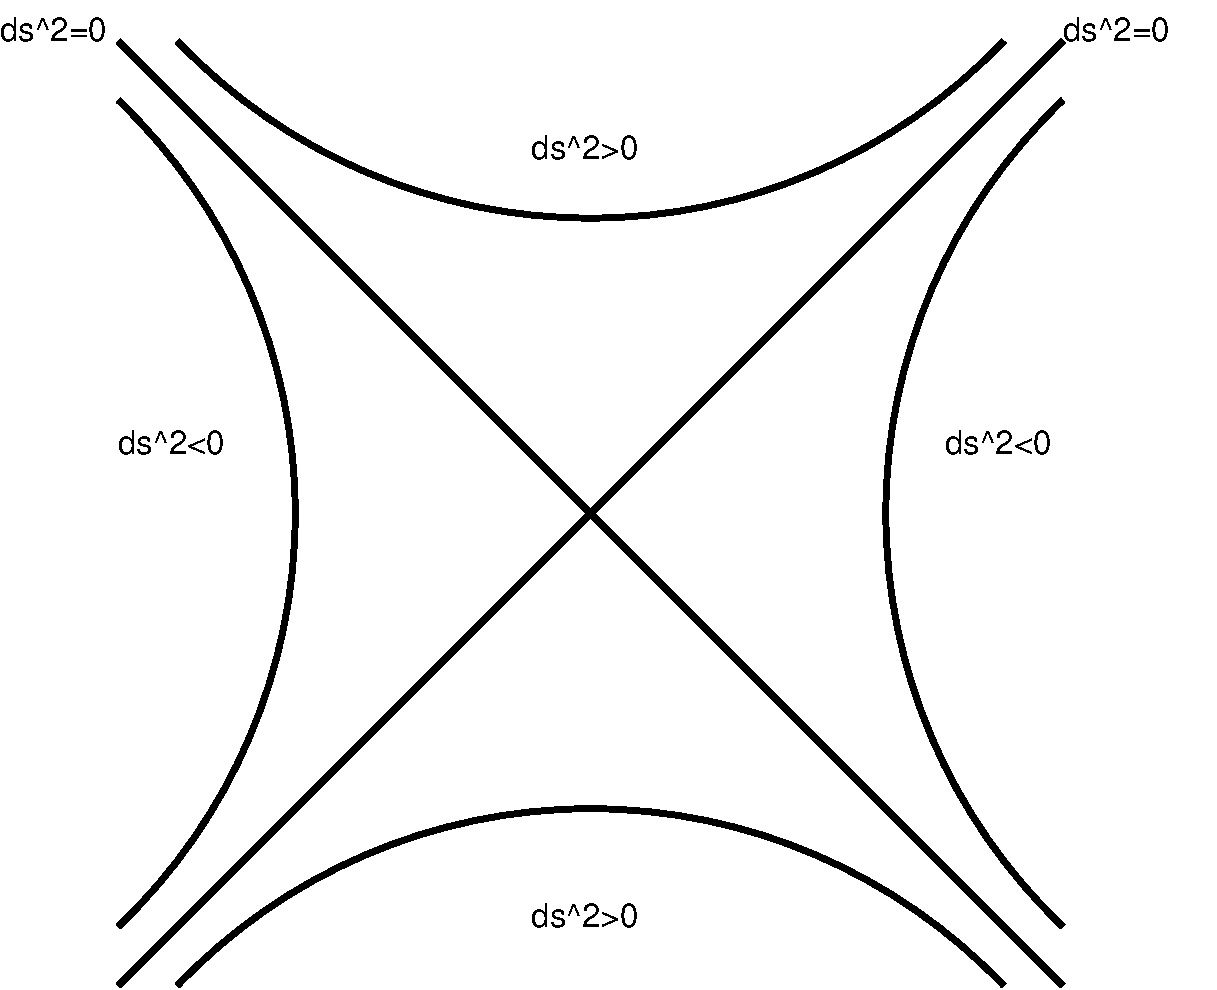
\includegraphics[width=6cm]{invariante.pdf}
    \caption{Come variano le iperboli al variare della costante}
    \label{fig:iperboli}
  \end{center}
\end{figure}

% Le ascisse sono rappresentate dalle $x$, e le ordinate sono
% rappresentate da $ct$.
Le iperboli sovrastanti gli asintoti, e sottostanti ad esse, sono
quelle con cost $>\,0$, e sono le uniche che possono verificarsi
(assieme agli asintoti), in quanto solo per esse vale
$\mathsf{v}<c$. Si giunge cos\`i alla rappresentazione del cono
\index{cono di luce}di luce di un punto (nel nostro caso, quello della
figura \vref{fig:cono}).
\begin{figure}[tb]
  \begin{center}
    \psfrag{ct per x=y=z=0}{\tiny $ct$ per $x=y=z=0$} \psfrag{B}{$B$}
    \psfrag{A}{$A$} \psfrag{D}{$D$} \psfrag{E}{$E$} \psfrag{x per
      ct=0}{\tiny $x$ per $c t=0$}
    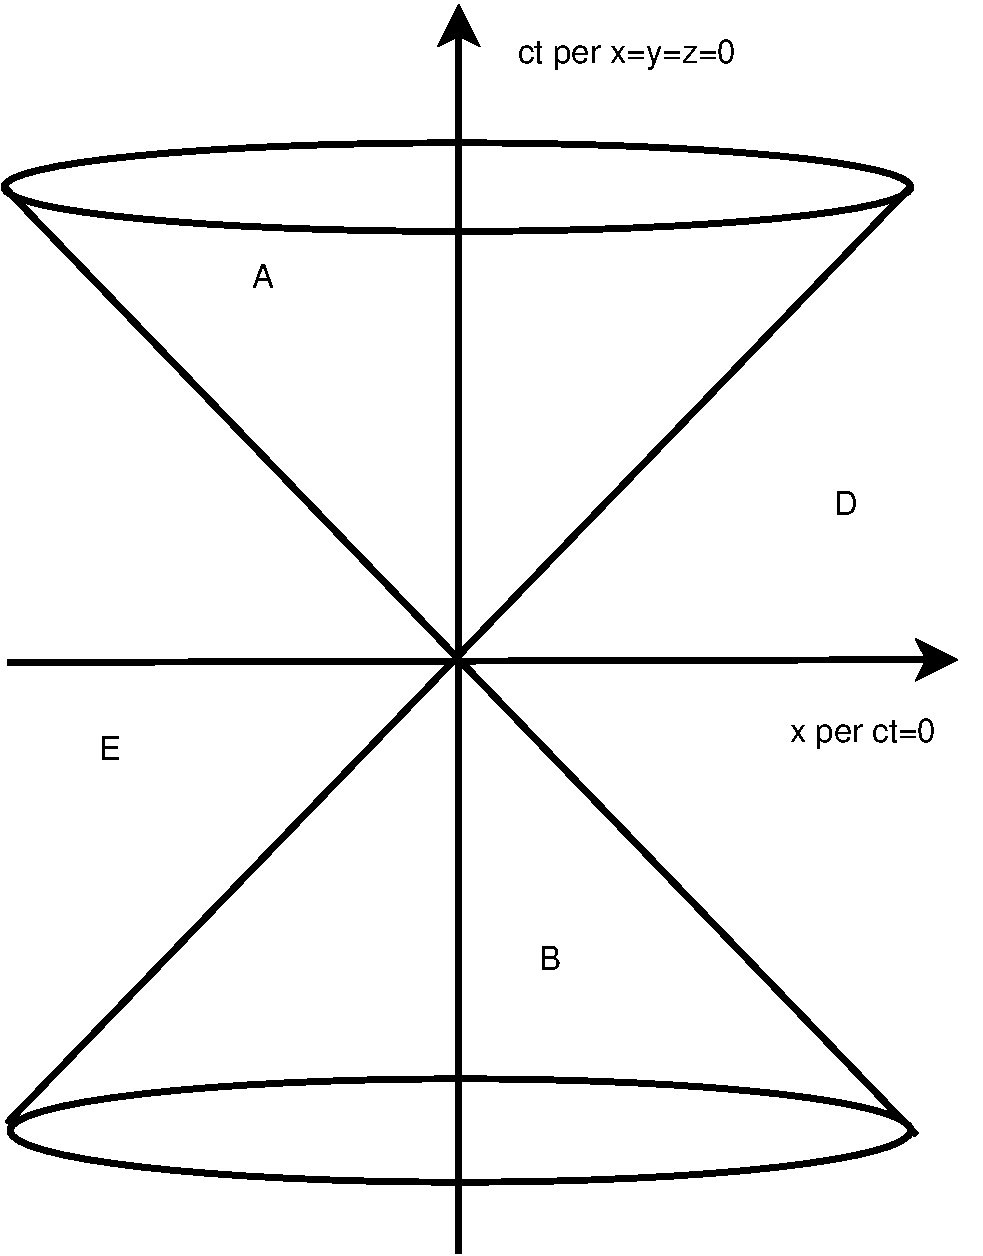
\includegraphics[width=6cm]{cono.pdf}
    \caption{Cono di luce} \label{fig:cono}
  \end{center}
\end{figure}
Cos'\`e questo cono di luce? Prendiamo due raggi di luce che si
propagano da $O$, nella direzione delle $x$, con verso opposto.  Essi
descriveranno la traiettoria che, se unita, dar\`a origine al semicono
superiore. Discorso analogo per due raggi di luce che arrivano
contemporaneamente in $0$: essi descriveranno il semicono
inferiore. L'unione di questi due semiconi viene detto cono di luce
(in quanto formato da raggi di luce.). Spieghiamo pi\`u in dettaglio
il vantaggio dell'introduzione del cono di luce.  Prendiamo gli eventi
$A$ e $B$ del diagramma in figura.  L'intervallo $\de s$ sar\`a
positivo. Poich\'e tale intervallo \`e invariante sotto trasformazioni
di Lorentz, qualsiasi altro sistema di riferimento vedr\`a tale
 intervallo positivo. Tali intervalli si dicono di tipo tempo (ogni
intervallo puramente temporale \`e infatti positivo.) Gli eventi
all'esterno del cono di luce saranno invece separati da intervalli
negativi, chiamati di tipo spazio. Agli eventi sulle bisettrici degli
assi saranno invece associati intervalli di tipo luce, pari ovvero a
0. \`E facile rendersi conto che gli eventi $D$ ed $E$ possono essere
contemporanei, in qualche opportuno sistema di riferimento. Gli altri
due eventi invece no. Per questo si dice che $A$ e $B$ stanno,
rispettivamente, nel cono del futuro e nel cono del passato, in quanto
appartegono al futuro \index{futuro assoluto}e al passato assoluti
\index{passato assoluto}dell'origine degli assi (a questo punto \`e
facile capire cosa voglia dire passato e futuro assoluti). Quindi,
guardando il cono di luce di un punto, \`e subito possibile capire
molte cose sulla ``sistemazione'' temporale dell'evento, in relazione
ad altri eventi.

Si capisce anche che eventi che non appartengono al futuro o passato
assoluto, non possono essere congiunti ad $O$ tramite traiettorie.
Questo si vede geometricamente considerando la tangente di tale
traiettoria, la quale risulterebbe minore di uno, ossia $ \frac{ c \de
  t }{ \de x} < 1 \Longrightarrow v > c$, assurdo.

\begin{osservazione}
  Possiamo a questo punto notare che il fatto di poter essere
  contemporanei implica che non \`e possibile che un'informazione che
  parte da uno di questi due eventi, possa raggiungere l'altro evento,
  in nessun sistema di riferimento, proprio perch\'e dovrebbe compiere
  una traiettoria con tangente (almeno in taluni punti), minore di
  uno. Questo rende conto della finitezza della velocit\`a di
  propagazione dell'informazione.
\end{osservazione}
\section{Relativo ed assoluto}
Ci proponiamo in questa sezione di analizzare, %
%prima da un punto di
%vista geometrico, e poi da un punto di vista algebrico, 
%cosa cambia e
%cosa rimane assoluto per quello che riguarda lunghezze e tempi.
come si comportano lunghezze e tempi nella teoria della relativit\`a
speciale: il punto cruciale risulter\`a nel trovare, ancora una volta,
risultati in netto contrasto con le nostre convinzioni.

\subsection{Quello che rimane assoluto}
\label{assoluto} Nel moto di un corpo visto da diversi osservatori
rimane assoluta l'immagine del corpo nello spazio tempo (ci\`o che
viene chiamato la sua linea di universo\index{linea di universo}).
%\begin{figure}[htbp]
%  \begin{center}
%    \psfrag{ct'}{$ct'$} \psfrag{ct}{$ct$} \psfrag{x'}{$x'$}
%    \psfrag{x}{$x$} \psfrag{O}{$O$} \psfrag{R}{$R$} \psfrag{R'}{$R'$}
%    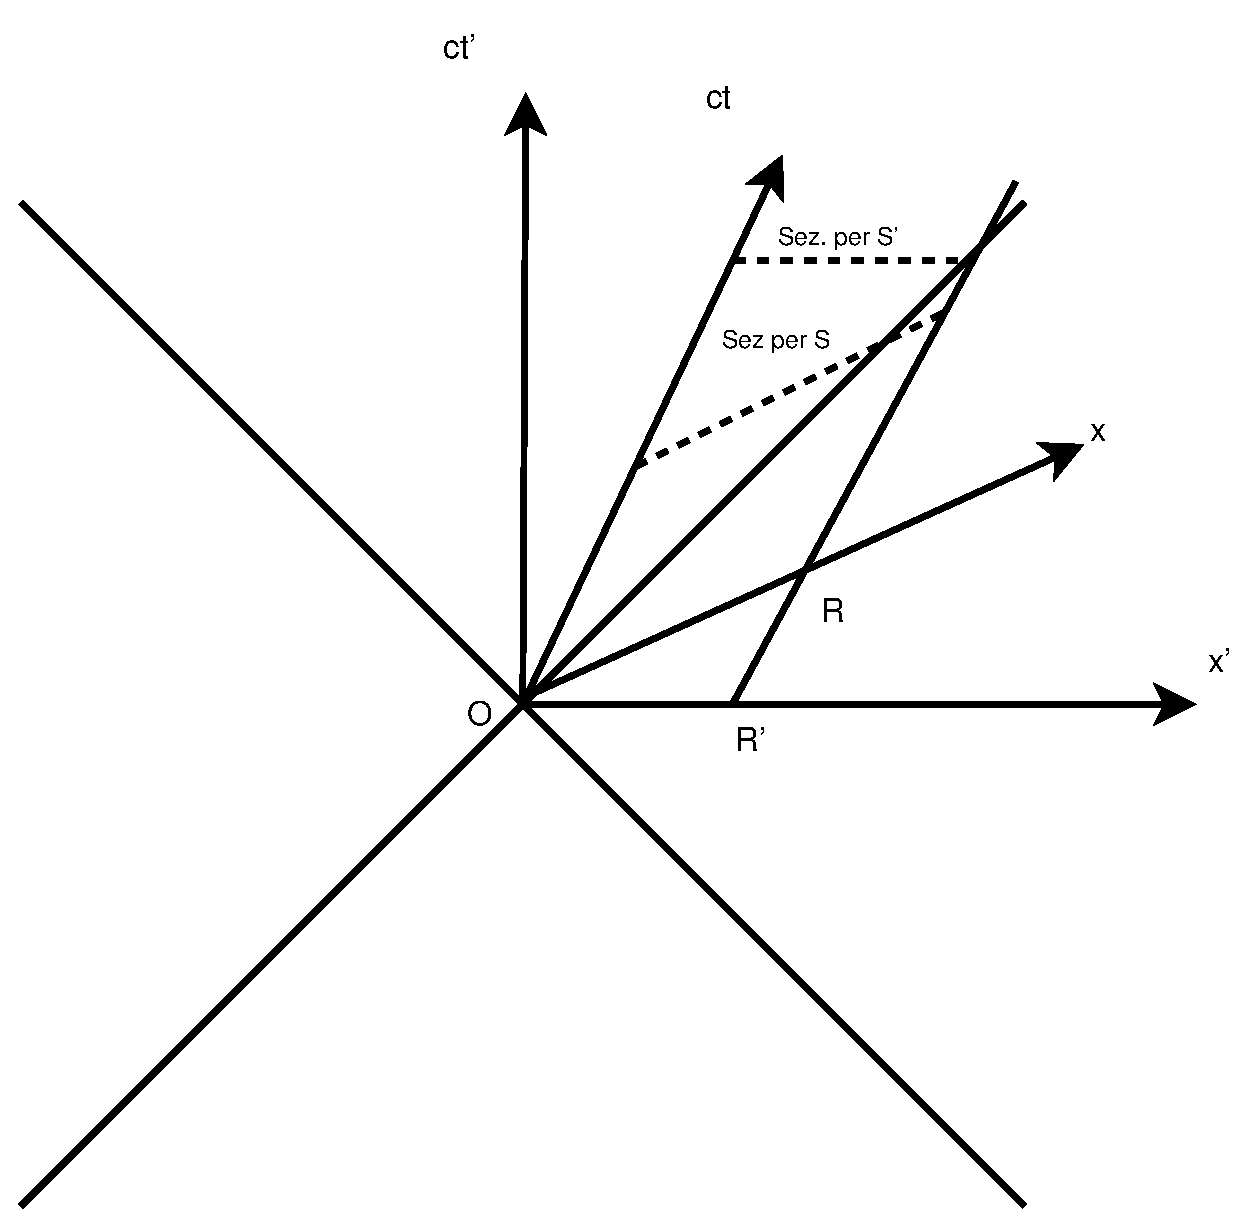
\includegraphics[height=8cm]{sezsbarra1.eps}
%    \caption{Ecco come l'immagine spazio temporale rimane la stessa
%      anche se vista da sistemi di riferimento in moto tra loro ($S$
%      ed $S'$ in questo caso)} \label{fig:Sez1}
%  \end{center}
%\end{figure}
Immaginiamo infatti di prendere un oggetto fermo nel sistema di
riferimento $S$, di assi $x$ e $ct$. Sia il corpo lungo un'unit\`a
(ragioniamo adimensionalmente, le cose non cambiano nella
sostanza). Se il corpo \`e lungo un'unit\`a, si ha:
\begin{equation}
  \mathbf{x}^2-(ct)^2\stackrel{t=0}{=}1\Longrightarrow
  \left[x\right]_{t=0}=1
\end{equation}
\begin{equation}
  \mbox{per cui } \forall t \qquad \mathbf{x}^2-(ct)^2=1
\end{equation}
e, dacch\'e questo \`e invariante, tutti gli osservatori vedono la
sbarra, \emph{nello spazio~tempo}, allo stesso modo in cui la vede
l'osservatore solidale alla sbarra, bench\'e \textbf{il modo in cui
  sia decomposta in spazio e tempo dipenda dall'osservatore.} Il fatto
che tempi e lunghezze siano ``distribuite'' in maniera diversa, si
ripercuote, portando alla contrazione di tempi e lunghezze.
\subsection{Contrazione lunghezze}
\index{contrazione delle lunghezze}
%Per analizzare la contrazione delle
%lunghezze riferiamoci alla figura \vref{fig:Sez2}; si ha:
%
%\begin{itemize} 
%\item $\overline{O'P'}=$ lunghezza 1 in $S'$\\
%\item $\overline{OP}=$ lunghezza 1 in $S$\\
%\item $\overline{O'R'}=$ lunghezza del regolo unitario a riposo in
%  $S$, misurata da $S'$\\
%\item $\overline{OR}=$ lunghezza del regolo unitario a riposo in
%      $S'$, misurata da $S$ \footnote{da qui si vede la contrazione
%        delle lunghezze: $\overline{O'R'}<\overline{O'P'}$ e
%        $\overline{OR}<\overline{OP}$}
%\end{itemize}
%
%\begin{figure}[htbp]
%  \begin{center}
%    \psfrag{ct'}{$ct'$} \psfrag{ct}{$ct$} \psfrag{x'}{$x'$}
%    \psfrag{x}{$x$} \psfrag{O}{$O$} \psfrag{R}{$R$} \psfrag{R'}{$R'$}
%    \psfrag{P}{$P$} \psfrag{P'}{$P'$}
%    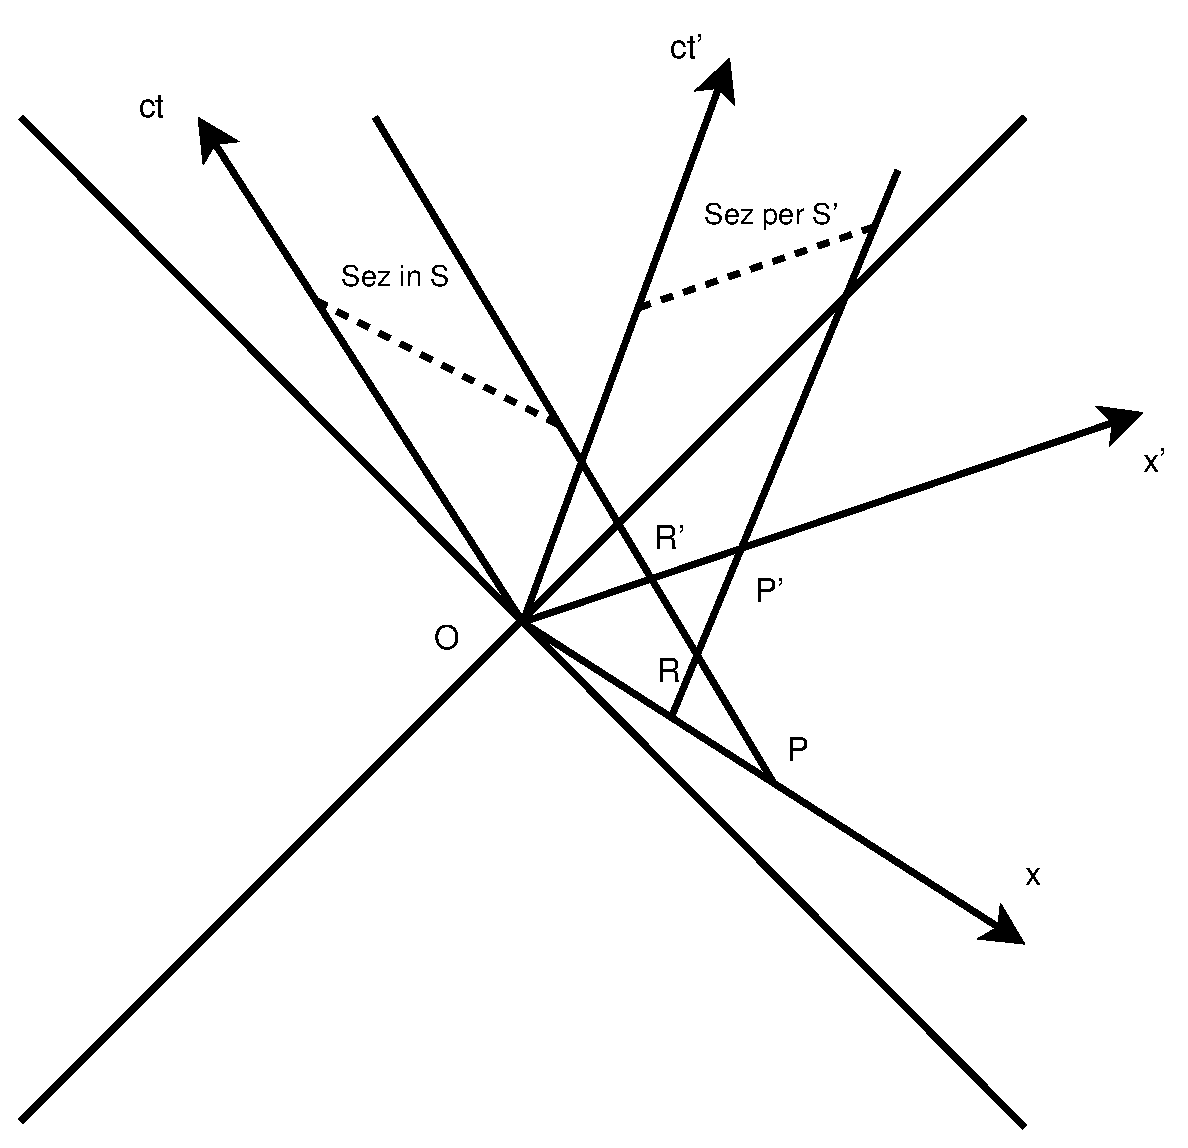
\includegraphics[height=8cm]{sezsbarra2.eps}
%    \caption{In figura si ha $OR$ ($OR'$) fotografia della sbarra
%      solidale a $S'$ ($S$) quando passa all'istante $0$ in $x$
%      ($x'$), $R'$ ($R$) \`e l'intersezione tra la sbarra in $x,c,t$
%      ($x',c',t'$) e l'asse $x'$ ($x$), $P'$ ($P$), punto dove
%      $[x']_{t'=0}=1$ ($[x]_{t=0}=1$). } \label{fig:Sez2}
%  \end{center}
%\end{figure}
%Mettiamo ora il tutto in formule, tramite le trasformazioni di Lorentz
%(\ref{eq:Lorentz}).
Per quel che riguarda la contrazione delle lunghezze, prendiamo la
 lunghezza del regolo unitario a riposo in $S'$, misurata da $S'$, pari
 a $\Delta x'$. Sia $\Delta x$ la lunghezza del regolo unitario a riposo
 in $S'$, misurata da $S$. Allora, tramite le trasformazioni di Lorentz (\ref{eq:Lorentz}):
\begin{displaymath}
  \Delta
  x'=x_{B}'-x_{A}'= \frac{x_{B} -
    \mathsf{v}t_{B}}{\sqrt{1-\frac{\mathsf{v}^2}{c^2}}} - \frac{x_{A}
    - \mathsf{v}t_{A}}{\sqrt{1-\frac{\mathsf{v}^2}{c^2}}}
\end{displaymath}
Se sono interessato alla misura effettuata da $S$, devo porre
$t_{A}=t_{B}$, e quindi:
\begin{displaymath}
  \Delta x=\Delta x'\cdot\sqrt{1-\frac{\mathsf{v}^2}{c^2}}<\Delta x'
\end{displaymath}
\subsection{Dilatazione dei tempi}
\index{dilatazione dei tempi} %Se vogliamo andare a vedere graficamente
%la dilatazione dei tempi procediamo riferendoci alla figura
%\vref{fig:Sez3}:
%\begin{figure}[htbp]
%  \begin{center}
%    \psfrag{ct'}{$ct'$} \psfrag{ct}{$ct$} \psfrag{x'}{$x'$}
%    \psfrag{x}{$x$} \psfrag{O}{$O$} \psfrag{R}{$R$} \psfrag{R'}{$R'$}
%    \psfrag{P}{$P$} \psfrag{P'}{$P'$}
%    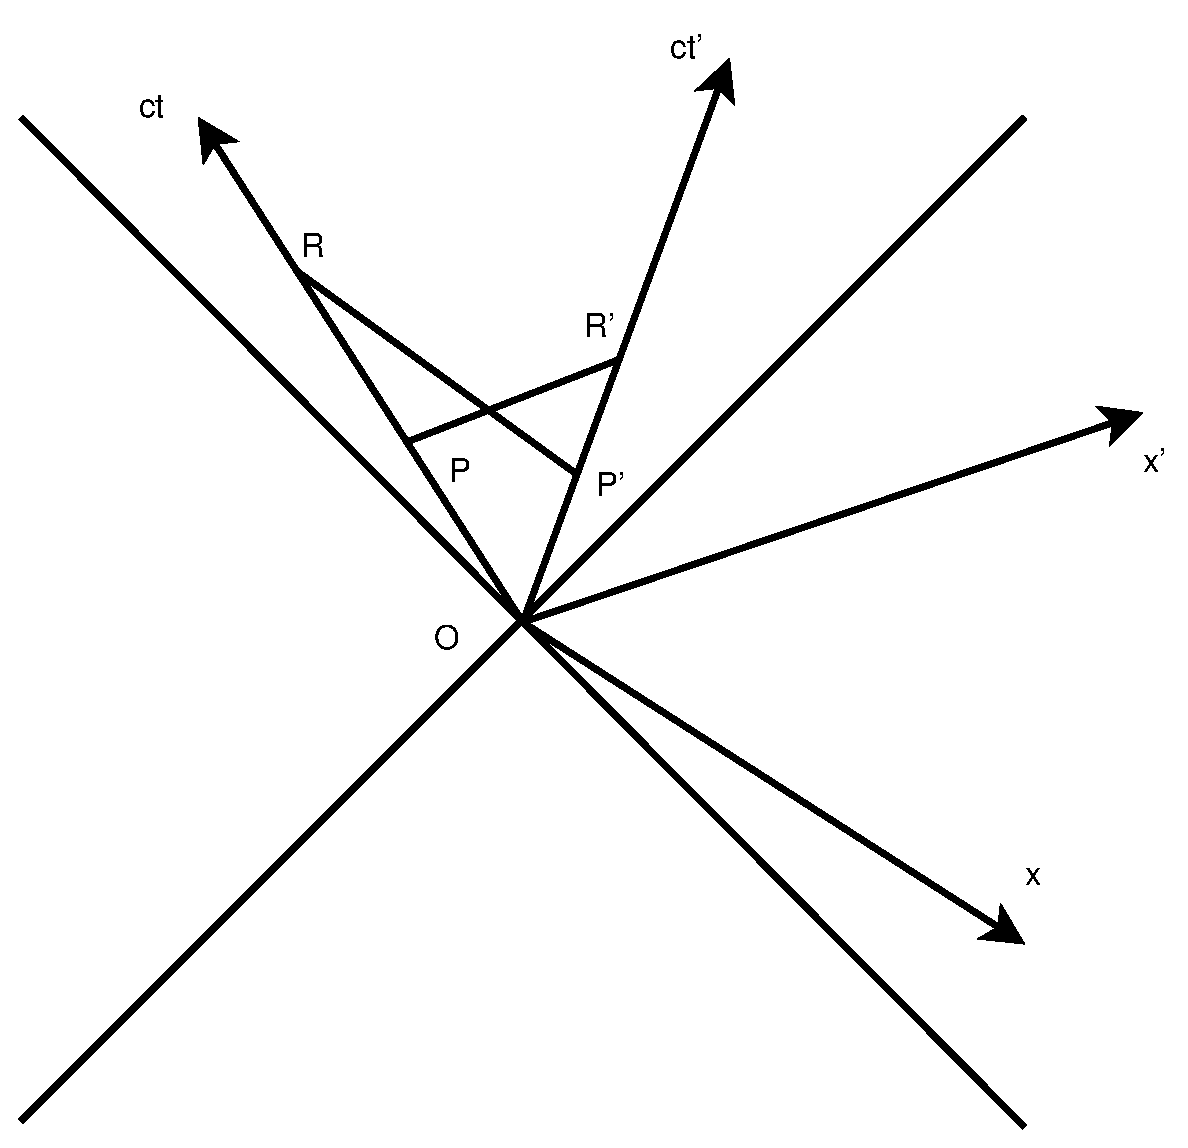
\includegraphics[height=8cm]{sezsbarra3.eps}
%    \caption{$R$ ($R'$) \`e il tempo simultaneo a $P'$ ($P$) in in $S$
%      ($S'$). $RP'$ ($R'P$) \`e segmento parallelo a $x'$
%      ($x$)}\label{fig:Sez3}
%  \end{center}
%\end{figure}
%\begin{itemize}
%\item $OP=$ tempo unitario di $S$ misurato da $S$\\
%\item $O'P'=$ tempo unitario di $S'$ misurato da $S'$\\ \item $O'R'=$
%  tempo unitario di $S$ misurato da $S'$\\
%\item $OR=$ tempo unitario di $S'$ misurato da $S$ \footnote{e da qui
%    la
%    dilatazione dei tempi: $O'R'>O'P'$ e $OR>OP$ }\\
%\end{itemize}
%Da qui si vede come i tempi ``cambiano'' a seconda del sistema di
%riferimento. Se vogliamo vedere il tutto in formule
Per vedere come i tempi sono ``influenzati'' da un cambio di sistema di
riferimento (\textbf{Attenzione: dobbiamo imporre che lo spazio sia lo
stesso se vogliamo andare a misurare i tempi}) prendiamo in
considerazione la misura del tempo di $S'$, fatta da $S$. Se voglio
misurare il tempo in $S'$, $\Delta x'$ deve essere $0$, come sopra
ricordato. Dunque:
\begin{displaymath}
\Delta t'=\frac{\Delta t-\frac{\mathsf{v}}{c^2}\Delta
  x}{\sqrt{1-\frac{\mathsf{v}^2}{c^2}}}
\end{displaymath}
\begin{displaymath}
\Delta x'=0=\frac{\Delta x-\mathsf{v}\Delta
  t}{\sqrt{1-\frac{\mathsf{v}^2}{c^2}}}
\end{displaymath}
\begin{displaymath}
\Longrightarrow \Delta x=\mathsf{v}\Delta t
\end{displaymath}
\begin{displaymath}
\Longrightarrow \Delta t'=\Delta t
\frac{1-\frac{\mathsf{v}^2}{c^2}}{\sqrt{1-\frac{\mathsf{v}^2}{c^2}}}=\Delta
t \sqrt{1-\frac{\mathsf{v}^2}{c^2}}
\end{displaymath}
\begin{displaymath}
\Longrightarrow\Delta t=\frac{\Delta
  t'}{\sqrt{1-\frac{\mathsf{v}^2}{c^2}}}>\Delta t'.
\end{displaymath}
Parlando di tempo, ci torner\`a molto utile introdurre il tempo
proprio, tramite la seguente
\begin{definizione}
  \index{tempo proprio}Il tempo proprio $\tau$ \`e il tempo misurato
  da un orologio in un sistema di riferimento in cui egli \`e fisso
  rispetto ad esso.
\end{definizione}

A noi risulter\`a comoda una definizione pi\`u ``operativa'', ovvero
si parler\`a di intervallo \index{intervallo!di tempo proprio}di tempo
proprio tra due eventi solidali al moto dell'orologio, come il tempo
necessario a quest'ultimo per misurare l'intervallo tra questi due
eventi, essendo questi fermi rispetto all'orologio; il quadrato
dell'intervallo spazio temporale avr\`a perci\`o la forma:
\begin{displaymath}
\de s^2 = c^2 \de \tau^2;
\end{displaymath}

in un altro sistema di riferimento invece
\begin{displaymath}
\de s^2 = c^2 \de t'^2 - \de \bef{x}^2=c^2 \de t'^2
(1-\frac{\bef{v^2}}{c^2}),
\end{displaymath}

il che implica $\de \tau = \de t' / \gamma$ e
\begin{displaymath}
\Delta \tau = \int_A^B \sqrt{1-\frac{\bef{v^2}}{c^2}} \de t'.
\end{displaymath}

\section{Considerazioni}
\begin{esempio}[Paradosso dei gemelli]
  A conferma di questo citiamo il famoso paradosso dei gemelli: uno
  dei due sale su un razzo con velocit\`a prossima alla velocit\`a
  della luce, l'altro rimane sulla terra. Quando quello che era sul
  razzo torna indietro risulta pi\`u giovane. Perch\'e? Considerando
  il diagramma spazio~tempo, ci accorgiamo che il sistema razzo ,
  quando esso torna verso la terra, cessa per un momento di essere
  inerziale (e se deve passare da velocit\`a prossime a~$c$ in una
  direzione, a velocit\`a prossime a~$c$ nell'altra direzione, dovr\`a
  accelerare di molto), quindi non possiamo utilizzare le
  trasformazioni della relativit\`a ristretta. Tuttavia, detto $\Delta
  \tau$ il tempo proprio del razzo, possiamo prendere:
  \begin{equation}
    \Delta \tau=(\Delta t)_{\rem{T}}\sqrt{1-\frac{\mathsf{v}^2}{c^2}}
    \label{eq:ingenua}
  \end{equation}
  Assumendo che la (\ref{eq:ingenua}) sia vera per intervalli
  infinitesimi, possiamo scrivere:
  \begin{equation}
    \de \tau=(\de
    t')_{\rem{T}}\sqrt{1-\frac{\mathsf{v}^2}{c^2}}\label{eq:ingenuabis}
  \end{equation}
  e questa \`e corretta se $\mathsf{v}$ varia nel tempo. Ora, anche se
  un punto $P'$ non \`e in moto uniforme rispetto al sistema $S$,
  possiamo considerare istante per istante (istanti $t$, non $t'$), il
  sistema di riferimento inerziale $S'(t)$, la cui velocit\`a coincide
  con quella di $P'$ all'istante $t$. Se ora consideriamo che il
  razzo, tornando indietro, passi da velocit\`a $\rem{\mathbf{v}}$ a
  velocit\`a $\rem{\mathbf{-v}}$ istantaneamente, si ha (poich\'e
  $\rem{v}$ \`e al quadrato nella formula):
  \begin{displaymath}
    t_{2}'-t_{1}'=(t_{2}-t_{1})\sqrt{1-\frac{\mathsf{v}^2}{c^2}}\:.
  \end{displaymath}

Questo risultato si rivela corretto, ma ci chiediamo: se siamo passati
istantaneamente da velocit\`a $\rem{\mathbf{v}}$ a velocit\`a
$\rem{\mathbf{-v}}$, perch\`e il gemello non vede le cose
simmetricamente rispetto al gemello sulla terra? Ovvero perch\'e egli
non vede che il gemello sulla terra \`e invecchiato della stessa
quantit\`a di quanto sia invecchiato lui? Il motivo sta nel fatto che
egli non pu\`o fare questo ragionamento (o meglio, pu\`o farlo, ma si
sbaglierebbe) poich\`e nell'inversione di velocit\`a lui cambia
sistema di riferimento, e quindi non \`e possibile applicare le
trasformazioni da noi trovate, in quanto esse valgono solo se non
cambiamo sistema di riferimento in itinere. Il gemello della terra
invece pu\`o sempre usarle, in quanto non cambia mai il proprio
sistema di riferimento.
\end{esempio}
\begin{esempio}[Decadimento $\Pi^{0}$]
  La prova sperimentale della teoria sopra esposta viene dagli
  acceleratori di particelle. Consideriamo ad esempio la particella
  neutra $\Pi^{{0}}$ (pione); quest'ultima nel suo sistema di
  riferimento (solidale alla particella) ha un tempo di vita medio
  $\tau=2\cdot 10^{-8}$s; cio\`e dopo un tempo $\tau$ il pione decade
  e si ha l'emissione di raggi gamma. $\Pi^{0}$ raggiunge una
  velocit\`a $v$ tale che $\beta \equiv \frac{v}{c}=0.99995$; quindi:
  \begin{displaymath}
    \tau'=\frac{\tau}{\sqrt{1-\beta^{2}}}=\tau \gamma \quad
    \textrm{dove}\;\frac{1}{\sqrt{1-\beta^{2}}}\equiv\gamma
  \end{displaymath}
  Si ha che $\gamma\simeq100$. Di conseguenza il tempo medio di vita
  che noi osserviamo \`e circa 100 volte superiore. Calcoliamo ora la
  distanza percorsa nell'acceleratore\index{acceleratore} da
  $\Pi^{0}$; essa sar\`a $L=v\tau\gamma\simeq600$m, mentre, non
  considerando gli effetti relativistici otteniamo $L=v\tau \simeq6$ m
  (fare bene attenzione per\`o: il $\Pi^{0}$ nel sistema di
  riferimento laboratorio decade dopo $600\,$m, ma nel suo sistema di
  riferimento vede lo spazio contratto, e quindi uguale a $ 600 \,
  \rem{ m } / \gamma = 6 \, \rem{ m }$); la differenza fra i due
  percorsi \`e bene osservabile. Aumentando la velocit\`a del pione se
  ne pu\`o aumentare il tempo di vita medio; in generale in questo
  modo sono possibili esperimenti anche su particelle che da ferme
  decadrebbero istantaneamente.
\end{esempio}
\section{Composizione delle velocit\`a}
\index{composizione delle velocit\`a}Consideriamo
$S^{\prime}$($x^{\prime}$,$t^{\prime}$) in moto rispetto ad
$S$($x$,$t$) con velocit\`a $v$ lungo $x$. Avremo quindi che:
\begin{displaymath}
  v^{\prime}_{x}=\frac{\de x^{\prime}}{\de t^{\prime}}=\frac{\de
    x-v\de
    t}{\sqrt{1-\frac{v^{2}}{c^{2}}}}\frac{\sqrt{1-\frac{v^{2}}{c^{2}}}}{\de
    t-\frac{v}{c^{2}}\de x}=\frac{\frac{\de x}{\de
      t}-v}{1-\frac{v}{c^{2}}\frac{\de x}{\de
      t}}=\frac{v_{x}-v}{1-\frac{v}{c^{2}}v_{x}}
\end{displaymath}
\begin{displaymath}
  v^{\prime}_{y}=\frac{\de y^{\prime}}{\de t^{\prime}}=\frac{\de
    y}{\de t-\frac{v}{c^{2}} \, \de
    x}\sq=\frac{v_{y}}{1-\frac{v}{c^{2}}v_{x}}\sq
\end{displaymath}
\begin{displaymath}
  v^{\prime}_{z}=\frac{v_{z}}{1-\frac{v}{c^{2}}v_{x}}\sq
\end{displaymath}
\begin{osservazione}
  Sfruttando le trasformazioni di Lorentz abbiamo ricavato le leggi di
  composizione delle velocit\`a; dobbiamo per\`o ancora verificare
  che:
  \begin{enumerate}
  \item se $v\ll c$ cio\`e $\frac{v}{c}\ll 1$ si ritorni ad avere la
    legge della composizione delle velocit\`a classica; tuttavia si
    verifica subito che:
    \begin{displaymath}
      v^{\prime}_{x}\simeq v_{x}-v\quad\textrm{quando}\;\frac{v}{c}\ll 1
    \end{displaymath}
    \begin{displaymath}
      v^{\prime}_{y}\simeq v_{y}
    \end{displaymath}
    \begin{displaymath}
      v^{\prime}_{z}\simeq v_{z}
    \end{displaymath}
  \item se $|v|=c$ ( dove $|v|=\sqrt{v_{x}^{2}+v_{y}^{2}+v_{z}^{2}}$ )
    allora anche $|v^{\prime}|=c$, dato che la velocit\`a della luce
    nel vuoto \`e la stessa per tutti i sistemi di riferimento
    inerziali. Nel caso in cui $v_{x}=c$, $v_{y}=0$, $v_{z}=0$ cio\`e
    che la luce si muova parallelamente a $v$ lungo $x$ si ha che:
    \begin{displaymath}
      v_{x}^{\prime} = 
      \frac{v_{x}-v}{1-\frac{v}{c^{2}}v_{x}}=\frac{c-v}{1-\frac{v}{c}}=c
    \end{displaymath}
    \begin{displaymath}
      v_{y}^{\prime}=0
    \end{displaymath}
    \begin{displaymath}
      v_{z}^{\prime}=0
    \end{displaymath}
    Un'altra possibilit\`a \`e il caso in cui la luce si muova
    perpendicolarmente a $v$ cio\`e: $v_{y}=c$ e $v_{x}=v_{z}=0$. Si
    ottiene:
    \begin{displaymath}
      v_{x}^{\prime}=\frac{v_{x}-v}{1-\frac{v}{c^{2}}v_{x}}=-v
    \end{displaymath}
    \begin{displaymath}
      v_{y}^{\prime}=\frac{v_{y}\sq}{1-\frac{v}{c^{2}}v_{x}}=c\sq
    \end{displaymath}
    \begin{displaymath}
      v_{z}^{\prime}=0
    \end{displaymath}
    Allora:
    \begin{displaymath}
      | v^{\prime}|=\sqrt{v^{2}+c^{2}(1-\frac{v^{2}}{c^{2}})}=c
    \end{displaymath}
  \end{enumerate}
\end{osservazione}
\section{Invarianza dell'intervallo spazio-temporale}
Cerchiamo in questa sezione di dare alcune nozioni sulle
trasformazioni che lasciano invariato l'intervallo
spazio-temporale. \`E una generalizzazione della struttura vettoriale
e dell'invarianza sotto rotazioni e traslazioni della meccanica
classica. Diamo ora una definizione importante, ed enunciamo e
dimostriamo in seguito un fondamentale teorema.
\begin{definizione}[Intervallo spazio-temporale]
  \index{intervallo!spazio-temporale} Detti $x^0 = t$, $x^1=x$,
  $x^2=y$, $x^3 =z $, definiamo la grandezza
  $s_{\rem{\scriptscriptstyle AB}}$ tale che:
  \begin{displaymath}
    s_{\rem{\scriptscriptstyle AB}}^2 = {(x_{\rem{\scriptscriptstyle
          A}}^0 - x_{\rem{\scriptscriptstyle B}}^0)}^2 -
    {(x_{\rem{\scriptscriptstyle A}}^1 - x_{\rem{\scriptscriptstyle
          B}}^1)}^2 - {(x_{\rem{\scriptscriptstyle A}}^2 -
      x_{\rem{\scriptscriptstyle B}}^2)}^2 -
    {(x_{\rem{\scriptscriptstyle A}}^3 - x_{\rem{\scriptscriptstyle
          B}}^3)}^2
  \end{displaymath}
  Chiaramente se $A$ e $B$ sono lungo una traiettoria di un raggio di
  luce, $s_{\rem{\scriptscriptstyle AB}} = 0$, mentre se $A$ e $B$
  sono lungo una traiettoria di una particella massiva, si ha $|
  \mathbf{ \rem{ v } } | < c \Longrightarrow
  s_{\rem{\scriptscriptstyle AB}} > 0$.
\end{definizione}
\begin{teorema}
  \index{teorema!dell'invarianza dell'intervallo} L'intervallo
  spazio-temporale tra due eventi \`e un invariante per trasformazioni
  tra sistemi di riferimento inerziali.
\end{teorema}
\begin{dimostrazione}Dimostriamo il tutto per intervalli infinitesimi,
  e poi estendiamo il nostro ragionamento a intervalli finiti; sia
  dunque $x_{\rem{\scriptscriptstyle B}}^{\mu} =
  x_{\rem{\scriptscriptstyle A}}^{\mu} + \de x^{ \mu }$\footnote{La
    lettera greca $\mu$ \`e un indice, che pu\`o assumere i valori da
    0 a 3.}, nel sistema di riferimento inerziale $S$; dobbiamo
  mostrare che:
  \begin{displaymath}
    \de s^2 = {(\de x^0)}^2 - {(\de x^1)}^2 - {(\de x^2)}^2 - {(\de
      x^3)}^2
  \end{displaymath}
  \`e invariante\footnote{Il modo in cui $\de s^2$ \`e stato scritto
    \`e impreciso: per i successivi sviluppi che faremo, sarebbe pi\`u
    opportuno scrivere $\de s^2 = \de x^0 \otimes \de x^0 - \de x^1
    \otimes \de x^1 - \de x^2 \otimes \de x^2 - \de x^3 \otimes \de
    x^3$, ma consci del fatto che solo gli studenti che hanno seguito
    il corso di Analisi delle Variet\`a Differenziali possono
    apprezzarlo, proseguiremo ignorando la nostra
    imprecisione.}. Prendiamo in considerazione un altro sistema di
  riferimento, sia esso $S'$; per passare da un sistema di coordinate
  all'altro si usi la funzione:
  \begin{displaymath}
    {x'}^{\mu} = f^{ \mu }( x )
  \end{displaymath}
  dove $f$ \`e una trasformazione che dipende da $\left( x^0 , x^1 ,
    x^2 , x^3 \right)$. Possiamo allora scrivere:
  \begin{equation}
    \de {x'}^{ \mu } = \sum_{\nu =0 }^{ 3 } \frac{ \partial f^{ \mu }(
      x ) }{ \partial x^{\nu} } \de x^{\nu} \label{eq:differenziale}
  \end{equation}
  La condizione di omogeneit\`a implica che $ \frac{ \partial f^{ \mu
    }( x ) }{ \partial x^{\nu} } $ sia costante, in quanto
  l'intervallo $\de {x'}^{ \mu}$ non pu\`o dipendere dal punto in cui
  mi trovo, per l'omogeneit\`a dello spazio. Pongo ora:
  \begin{displaymath}
    \frac{\partial f^{ \mu }( x ) }{ \partial x^{\nu} } := \la^{ \mu} {}_{ \nu }.
  \end{displaymath}
  Integrando la (\ref{eq:differenziale}), ottengo:
  \begin{displaymath}
    {x'}^{ \mu} = \sum_{ \nu = 0}^{ 3 } \la^{ \mu } {}_{ \nu } x^{\nu}
    + a^{ \nu },
  \end{displaymath}
  con $ a $ costante. Posso dunque scrivere:
  \begin{displaymath}
    \de {s'}^{ 2 } = {(\de {x'}^{ 0 })}^2 - {( \de {\mathbf{ x }}'
      )}^2 = \sum_{ \mu,\nu = 0}^{ 3 } \left[ \la^0 {}_{\mu} \la^0
      {}_{\nu} - \sum_{i = 1}^{ 3 } \la^i {}_{\mu} \la^i {}_{\nu}
    \right] \de x^{ \mu } \de x^{ \nu }.
  \end{displaymath}
  Definisco ora:
  \begin{displaymath}
    g_{ \mu \nu } := \la^0 {}_{\mu} \la^0 {}_{\nu} -
    \sum_{i = 1}^{ 3 } \la^i {}_{\mu} \la^i {}_{\nu} \quad
    \mbox{\scriptsize (Osserviamo che \`e simmetrico)}
  \end{displaymath}
  Allora si ha:
  \begin{displaymath}
    \de {s'}^{ 2 }= \sum_{ \mu,\nu = 0 }^{3} g_{\mu \nu} \de x^{\mu}
    \de x^{\nu}.
  \end{displaymath}
  Considero ora un raggio di luce che si propaga in $S$ lungo $x$, il
  che implica $ \de y = \de z = 0 $. Allora:
  \begin{equation}
    0 \stackrel{\rem{\scriptscriptstyle raggio \;di\; luce}}{=} (\de
    {s'})^2 = g_{00} (\de x^0)^2 + 2 g_{01} \de x^1 \de x^0 + g_{11}
    (\de x^1)^2 
    \label{eq:gmunu}
  \end{equation}
  \begin{displaymath}
    g_{01}=g_{10} \;\;\mbox{\scriptsize poich\'e simmetrico;}
  \end{displaymath}
  poi:
  \begin{displaymath}
    {\de s}^2 = {(\de x^0)}^2 - {(\de x^1)}^2 = 0 \Longrightarrow \de
    x^0 = \de x^1.
  \end{displaymath}
  Allora la (\ref{eq:gmunu}) d\`a:
  \begin{equation}
    0 = {(\de s')}^2 = (g_{00} + g_{11} + 2 g_{10}){(\de x^0)}^2;
  \end{equation}
  Se il raggio di luce si propaga nella direzione opposta, $\de x^1$
  cambia segno e dunque:
  \begin{displaymath}
    0 = {(\de s')}^2 = (g_{00} + g_{11} - 2 g_{10}){(\de x^0)}^2
  \end{displaymath}
  il che implica $ 2 g_{10} = -2 g_{10}$, e tale relazione vale se
  solo se $ g_{10} = 0$. Questo ci permette di scrivere:
  \begin{displaymath}
    0 = (g_{00} + g_{11} + 2 g_{10}) = g_{00} + g_{11} \Longrightarrow
    g_{00} = - g_{11}
  \end{displaymath}
  Per l'isotropia dello spazio, il raggio di luce potevo sceglierlo
  propagantesi anche lungo $y$ o lungo $z$, il che permette di
  concludere:
  \begin{displaymath}
    - g_{00} = g_{11} = g_{22} = g_{33}
  \end{displaymath}
  \begin{displaymath}
    g_{01} = g_{02} = g_{03} = g_{10} = g_{20} =g_{30} = 0
  \end{displaymath}

  Considero adesso un raggio di luce generico:
  \begin{displaymath}
    0 = {(\de s')}^2 = g_{00}{(\de x^0)}^2 + g_{11}{(\de x^1)}^2 +
    g_{22}{(\de x^2)}^2 + g_{33}{(\de x^3)}^2 +
    \sum_{\stackrel{i,j=1}{i\neq j}}^{3} g_{ij} \de x^j \de x^i =
  \end{displaymath}
  \begin{displaymath}
    g_{00}{(\de s)}^2 + \sum_{\stackrel{i,j=1}{i\neq j}}^{3} g_{ij}
    \de x^j \de x^i = 0 + \sum_{\stackrel{i,j=1}{i\neq j}}^{3} g_{ij}
    \de x^j \de x^i \Longrightarrow g_{ij} = 0 \mbox{ se } i \neq j
  \end{displaymath}
  Questo comporta:
  \begin{equation} {(\de s')}^2 = g_{00} {(\de
      s)}^2; 
    \label{eq:essecongi}
  \end{equation}
  domandiamoci a questo punto quanto possa valere $g_{00}$. Tale
  oggetto non pu\`o dipendere da $x$, per l'omogeneit\`a; potrebbe poi
  dipendere da $|\mathbf{v}|$, ma non da $\mathbf{v}$, per l'isotropia
  $\Longrightarrow g_{00} = g_{00}(|\mathbf{v}|)$; se scambio il ruolo
  di $S$ e di $S'$, avremo che l'unica cosa che cambia \`e
  $\mathbf{v}$ in $-\mathbf{v}$; allora:
\begin{displaymath}
\de s^2 = g_{00} (|-\mathbf{v}|)\de {s'}^2 = g_{00} (|\mathbf{v}|)\de
{s'}^2 \stackrel{(\ref{eq:essecongi})}{=} g_{00}^2 (|\mathbf{v}|)\de
{s}^2 
\end{displaymath}
\begin{displaymath}
\Longrightarrow 1 = g_{00}^2 \Longrightarrow g_{00} = \pm 1; \mbox{ se
} \mathbf{v} = 0, g_{00} = 1,
\end{displaymath}
allora $g_{00}$ \`e sempre 1, dunque $\de s^2 = \de {s'}^2$ e
\begin{displaymath}
  g_{\mu \nu}=\left(
    \begin{array}{rrrr}
      1&0&0&0\\0&-1&0&0\\0&0&-1&0\\0&0&0&-1\\
    \end{array}
  \right)
\end{displaymath}
\end{dimostrazione}
